% This work is licensed under the Creative Commons
% Attribution-NonCommercial-ShareAlike 4.0 International License. To view a copy
% of this license, visit http://creativecommons.org/licenses/by-nc-sa/4.0/ or
% send a letter to Creative Commons, PO Box 1866, Mountain View, CA 94042, USA.

\documentclass[12pt,a4paper]{article} 

% This work is licensed under the Creative Commons
% Attribution-NonCommercial-ShareAlike 4.0 International License. To view a copy
% of this license, visit http://creativecommons.org/licenses/by-nc-sa/4.0/ or
% send a letter to Creative Commons, PO Box 1866, Mountain View, CA 94042, USA.

% PACKAGES
\usepackage[english, ngerman]{babel}	% Paket für Sprachselektion, in diesem Fall für deutsches Datum etc
\usepackage[utf8]{inputenc}	% Paket für Umlaute; verwende utf8 Kodierung in TexWorks 
\usepackage[T1]{fontenc} % ö,ü,ä werden richtig kodiert
\usepackage{amsmath} % wichtig für align-Umgebung
\usepackage{amssymb} % wichtig für \mathbb{} usw.
\usepackage{amsthm} % damit kann man eigene Theorem-Umgebungen definieren, proof-Umgebungen, etc.
\usepackage{mathrsfs} % für \mathscr
\usepackage[backref]{hyperref} % Inhaltsverzeichnis und \ref-Befehle werden in der PDF-klickbar
\usepackage[english, ngerman, capitalise]{cleveref}
\usepackage{graphicx}
\usepackage{grffile}
\usepackage{setspace} % wichtig für Lesbarkeit. Schöne Zeilenabstände

\usepackage{enumitem} % für custom Liste mit default Buchstaben
\usepackage{ulem} % für bessere Unterstreichung
\usepackage{contour} % für bessere Unterstreichung
\usepackage{epigraph} % für das coole Zitat

\usepackage{tikz}

% This work is licensed under the Creative Commons
% Attribution-NonCommercial-ShareAlike 4.0 International License. To view a copy
% of this license, visit http://creativecommons.org/licenses/by-nc-sa/4.0/ or
% send a letter to Creative Commons, PO Box 1866, Mountain View, CA 94042, USA.

% THEOREM-ENVIRONMENTS

\newtheoremstyle{mystyle}
  {20pt}   % ABOVESPACE \topsep is default, 20pt looks nice
  {20pt}   % BELOWSPACE \topsep is default, 20pt looks nice
  {\normalfont} % BODYFONT
  {0pt}       % INDENT (empty value is the same as 0pt)
  {\bfseries} % HEADFONT
  {}          % HEADPUNCT (if needed)
  {5pt plus 1pt minus 1pt} % HEADSPACE
	{}          % CUSTOM-HEAD-SPEC
\theoremstyle{mystyle}

% Definitionen der Satz, Lemma... - Umgebungen. Der Zähler von "satz" ist dem "section"-Zähler untergeordnet, alle weiteren Umgebungen bedienen sich des satz-Zählers.
\newtheorem{satz}{Satz}[section]
\newtheorem{lemma}[satz]{Lemma}
\newtheorem{korollar}[satz]{Korollar}
\newtheorem{proposition}[satz]{Proposition}
\newtheorem{beispiel}[satz]{Beispiel}
\newtheorem{definition}[satz]{Definition}
\newtheorem{bemerkungnr}[satz]{Bemerkung}
\newtheorem{theorem}[satz]{Theorem}

% Bemerkungen, Erinnerungen und Notationshinweise werden ohne Numerierungen dargestellt.
\newtheorem*{bemerkung}{Bemerkung.}
\newtheorem*{erinnerung}{Erinnerung.}
\newtheorem*{notation}{Notation.}
\newtheorem*{aufgabe}{Aufgabe.}
\newtheorem*{lösung}{Lösung.}
\newtheorem*{beisp}{Beispiel.} %Beispiel ohne Nummerierung
\newtheorem*{defi}{Definition.} %Definition ohne Nummerierung
\newtheorem*{lem}{Lemma.} %Lemma ohne Nummerierung


% SHORTCUTS
\newcommand{\R}{\mathbb{R}}				 % reelle Zahlen
\newcommand{\Rn}{\R^n}						 % der R^n
\newcommand{\N}{\mathbb{N}}				 % natürliche Zahlen
\newcommand{\Z}{\mathbb{Z}}				 % ganze Zahlen
\newcommand{\C}{\mathbb{C}}			   % komplexe Zahlen
\newcommand{\gdw}{\Leftrightarrow} % Genau dann, wenn
\newcommand{\with}{\text{ mit }}   % mit
\newcommand{\falls}{\text{falls }} % falls
\newcommand{\dd}{\text{ d}}        % Differential d

% ETWAS SPEZIELLERE ZEICHEN
%disjoint union
\newcommand{\bigcupdot}{
	\mathop{\vphantom{\bigcup}\mathpalette\setbigcupdot\cdot}\displaylimits
}
\newcommand{\setbigcupdot}[2]{\ooalign{\hfil$#1\bigcup$\hfil\cr\hfil$#2$\hfil\cr\cr}}
%big times
\newcommand*{\bigtimes}{\mathop{\raisebox{-.5ex}{\hbox{\huge{$\times$}}}}} 

% WHITESPACE COMMANDS
%non-restrict newline command
\newcommand{\enter}{$ $\newline} 
%praktischer Tabulator
\newcommand\tab[1][1cm]{\hspace*{#1}}

% TEXT ÜBER ZEICHEN
%das ist ein Gleichheitszeichen mit Text darüber, Beispiel: $a\stackeq{Def} b$
\newcommand{\stackeq}[1]{
	\mathrel{\stackrel{\makebox[0pt]{\mbox{\normalfont\tiny #1}}}{=}}
} 
%das ist ein beliebiges Zeichen mit Text darüber, z. B.  $a\stackrel{Def}{\Rightarrow} b$
\newcommand{\stacksymbol}[2]{
	\mathrel{\stackrel{\makebox[0pt]{\mbox{\normalfont\tiny #1}}}{#2}}
} 

% UNDERLINE
% besseres underline 
\renewcommand{\ULdepth}{1pt}
\contourlength{0.5pt}
\newcommand{\ul}[1]{
	\uline{\phantom{#1}}\llap{\contour{white}{#1}}
}


% hier noch ein paar Commands die nur ich nutze, weil ich sie mir im Laufe der Jahre angewöhnt habe und sie mir jetzt nicht abgewöhnen will:

\newcommand{\gdw}{\Leftrightarrow}   % genau dann, wenn



% Commands für Stochastik / Statistik
\newcommand{\A}{\mathcal{A}}
\renewcommand{\P}{\mathbb{P}}
\newcommand{\E}{\mathbb{E}}




% This work is licensed under the Creative Commons
% Attribution-NonCommercial-ShareAlike 4.0 International License. To view a copy
% of this license, visit http://creativecommons.org/licenses/by-nc-sa/4.0/ or
% send a letter to Creative Commons, PO Box 1866, Mountain View, CA 94042, USA.

% Commands für WTHM
\newcommand{\F}{\mathcal{F}}				% Standard-Unter-Sigma-Algebra / Filtration
\newcommand{\G}{\mathcal{G}}				% Gegenstück zu \F für Rückwärtsmartingale

% independent symbol from:
% https://tex.stackexchange.com/questions/79434/double-perpendicular-symbol-for-independence
\newcommand{\unab}{\protect\mathpalette{\protect\independenT}{\perp}}
\def\independenT#1#2{\mathrel{\rlap{$#1#2$}\mkern2mu{#1#2}}}

\newcommand{\BedE}[2]{\E\left[{#1}~|~{#2}\right]} % Bedingte Erwartung
\newcommand{\graph}{\text{graph}}

%\newcommand{\binom}[2]{\begin{pmatrix}	{#1}\\{#2} \end{pmatrix}} %this command doesn't compile for me




\author{Willi Sontopski}

\parindent0cm %Ist wichtig, um führende Leerzeichen zu entfernen

\usepackage{color}

\usepackage{scrpage2}
\pagestyle{scrheadings}
\clearscrheadfoot

\ihead{Willi Sontopski}
\chead{WTHM WiSe 18 19}
\ohead{}
\ifoot{Aufgabenblatt 3}
\cfoot{Version: \today}
\ofoot{Seite \pagemark}

\begin{document}
%\setcounter{section}{1}

\section*{Aufgabe 1}
Seien $\sigma,\tau$ Stoppzeiten bzgl. der Filtration $(\F_n)_{n\in\N}$ und $\F_\tau$ definiert durch
\begin{align*}
\F_\tau:=\big\lbrace A\in\A~\big|~\forall n\in\N_0:A\cap\lbrace\tau\leq n\rbrace\in\F_n\big\rbrace
\end{align*}
Dann gilt:
\begin{enumerate}[label=\alph*)]
\item $\F_\tau$ ist eine $\sigma$-Algebra
\item $\begin{aligned}
\sigma\leq\tau\implies\F_\sigma\subseteq\F_\tau
\end{aligned}$
\item $\begin{aligned}
\lbrace\tau\leq\sigma\rbrace\in\F_\tau\cap\F_\sigma
\end{aligned}$
\item $\begin{aligned}
\F_\tau\cap\F_\sigma=\F_{\tau\wedge\sigma}
\end{aligned}$
\end{enumerate}
\begin{proof}[Beweis von Willi.]\enter
\underline{Zeige a):} Sei $n\in\N_0$ beliebig aber fest.
\begin{itemize} 
\item $\Omega\in\F_\tau$, denn $\Omega\in\A$ und 
\begin{align*}
\Omega\cap\lbrace\tau\leq n\rbrace=\lbrace\tau\leq n\rbrace \stackrel{\text{SZ}}{\in} \F_n
\end{align*}
\item Sei $A \in \F_\tau$. Dann gilt $A^C \in \F_\tau$, denn:\\
\begin{align*}
\lbrace\tau\leq n\rbrace &=\big(\lbrace\tau\leq n\rbrace\cap A\big)\dot{\cup}\big(\lbrace\tau\leq n\rbrace\cap A^C\big)\\
\implies A^C\cap\lbrace\tau\leq n\rbrace&=\underbrace{\lbrace\tau\leq n\rbrace}_{\stackrel{\text{SZ}}{\in}\F_n}\setminus\big(\underbrace{\lbrace\tau\leq n\rbrace\cap A\big)}_{\stackrel{\text{Vor}}{\in}\F_n}\stackrel{\sigma\text{A}}{\in}\F_n
\end{align*}
Alternative: Sei $A \in \F_\tau$
\begin{align*}
	A^C\cap \lbrace \tau \leq n \rbrace = \left(\underbrace{A}_{\stackrel{\text{Vor.}}{\in} \F_n} \cup \underbrace{\lbrace \tau \leq n \rbrace^C}_{\stackrel{\sigma\text{-Alg}}{\in} \F_n} \right)^C \stackrel{\sigma\text{-Alg}}{\in}\F_n
\end{align*}

\item Sei $(A_i)_{i\in\N}\subseteq\F_\tau$. Dann gilt $\bigcup\limits_{i\in\N} A_i  \in \F_\tau$, denn:\\
Offenbar ist $\bigcup\limits_{i\in\N} A_i  \in\A$ und nach Voraussetzung gilt $A_i\in\A$ und\\ $A_i\cap\lbrace\tau\leq n\rbrace\in\F_n~\forall i\in\N_0$. Folglich gilt:
\begin{align*}
\underbrace{\bigcup\limits_{i=1}^{\infty} \Big (A_i \cap \{\tau \leq n\} \Big )}_{\stackrel{\sigma\text{A}}{\in} \F_n} = \left( \bigcup\limits_{i=1}^{\infty} A_i \right)\cap \{\tau \leq n\} \implies  \bigcup\limits_{i=1}^{\infty} A_i \in \F_\tau
\end{align*}
\end{itemize}

\underline{Zeige b):}\\
Sei $A\in\F_\sigma$. Dann ist $A\in\A$ und $A\cap\lbrace\sigma\leq n\rbrace\in\F_n\forall n\in\N_0.$ Also gilt:
\begin{align*}
A \cap \lbrace\tau \leq n\rbrace
\stackeq{}
\big(A \cap\lbrace\tau \leq n\rbrace\big)\cap\underbrace{\lbrace\sigma\leq\tau\rbrace}_{\stackeq{\text{Vor.}}\Omega}
=\underbrace{A\cap\lbrace\sigma\leq n\rbrace}_{\stackrel{\text{Vor}}{\in}\F_n}\cap\underbrace{\lbrace\tau\leq n\rbrace}_{\stackrel{\text{SZ}}{\in}\F_n} \stackrel{\sigma\text{A}}{\in} \F_n \quad \forall n \in \N_0\\
\implies A\in\F_\tau
\end{align*}

\underline{Zeige c):}\\
Es ist ausreichend folgende zwei Aussagen zu zeigen:
\begin{align*}
	\lbrace \tau \leq \sigma\rbrace &\cap \lbrace \tau \leq n\rbrace \in \F_n &(\ast)&\\
	\lbrace \tau \leq \sigma\rbrace &\cap \lbrace \sigma \leq n\rbrace \in \F_n &(\ast\ast)& \\
\end{align*}

Zu $(\ast)$:
\begin{align*}
	&\lbrace \tau \leq \sigma\rbrace \cap \lbrace \tau \leq n\rbrace\\
	=&\lbrace \tau \leq \min\{\sigma, n\}\rbrace  \\
	=&\lbrace \tau \leq \min\{\sigma, n\}, \sigma \geq n\rbrace \cup 
	\lbrace \tau \leq \min\{\sigma, n\}, \sigma < n\rbrace \\
	=&\underbrace{\lbrace \tau \leq n\rbrace}_{\in \F_n} \cup
	\underbrace{\lbrace \tau \leq \sigma, \sigma < n\rbrace}_{\in \F_\sigma \subset \F_n} \in \F_n \\
\end{align*}

Zu $(\ast\ast)$:
Verläuft ähnlich wie der letzte Schritt in $(\ast)$:
\begin{align*}
	&\lbrace \tau \leq \sigma\rbrace \cap \lbrace \sigma \leq n\rbrace \\
	&=\underbrace{\lbrace \tau \leq \sigma, \sigma \leq n\rbrace}_{\F_\sigma \subset F_n} \in F_n \\
\end{align*}



\underline{Zeige d):}\\
\begin{itemize}
\item Zeige ``$\subseteq$'':
Sei $A\in\F_\tau\cap\F_\sigma$. Dann ist $A\in\A$ und
\begin{align*}
\big(A\cap\lbrace\tau\leq n\rbrace\big),\big(A\cap\lbrace\sigma\leq n\rbrace\big)\in\F_n\qquad\forall n\in\N_0
\end{align*}
Da $\F_n$ eine $\sigma$-Algebra ist, ist auch die Vereinigung enthalten:
\begin{align*}
&\big(A\cap\lbrace\tau\leq n\rbrace\big)\cup\big(A\cap\lbrace\sigma\leq n\rbrace\big)\in\F_n\\
&\implies
\big(A\cap\lbrace\tau\leq n\rbrace\big)\cup\big(A\cap\lbrace\sigma\leq n\rbrace\big)
&=&A\cap\big(\lbrace\tau\leq n\rbrace\cup\lbrace\sigma\leq n\rbrace\big)\\
&&=&A\cap\lbrace\tau\wedge\sigma\leq n\rbrace\in\F_n\\
&\implies A\in\F_{\sigma\wedge\tau}\implies \F_\tau\cap\F_\sigma\subseteq\F_{\tau\wedge\sigma}
\end{align*}

\item Zeige ``$\supseteq$'':
\begin{align*}
\tau\wedge\sigma\stackrel{\text{Def}}{\leq}\tau,\sigma\stackrel{\text{(b)}}{\implies}\F_{\sigma\wedge\tau}\subseteq\F_\tau,\F_\sigma\implies\F_{\tau\wedge\sigma}\subseteq\F_\tau\cap\F_\sigma
\end{align*}
\end{itemize}
\end{proof}

\begin{proof}[Beweis von Henrik.]\enter
\underline{Zeige a):}\\
\begin{itemize} 
	\item z.z.:$\emptyset \in \F_\tau$\\
	\begin{equation*}
		\emptyset \in \A \text{ und } \emptyset \in \F_n\  \forall n \in \N_0 \implies \emptyset \cap \{\tau \leq n\} \in \F_n
	\end{equation*}
	\item z.z.: $A \in \F_\tau \implies A^C \in \F_\tau$\\
	Sei $A \in \F_\tau$, d.h.:
	\begin{align*}
		&{}\qquad \quad  A \cap \{\tau \leq n\} \in \F_n \quad \forall n \in \N\\
		&\implies	A^C \cup \{\tau > n\} \in \F_n \quad \forall n \in \N\\
		&\implies 	\left(	A^C \cup \{\tau > n\}\right) \cap \{\tau \leq n\} \in \F_n \quad \forall n \in \N\\
		& \iff \left(	A^C \cap \{\tau \leq n\}\right) \cup \underbrace{\big ( \{\tau > n\}\cap\{\tau \leq n\} \big )}_{= \emptyset} \in \F_n \quad \forall n \in \N\\
		&\implies A^C \cap \{\tau \leq n\} \in \F_n \quad \forall n \in \N
	\end{align*}
	
	\item z.z.: Sei $A_1, A_2,\dots \in \F_\tau \implies \bigcup\limits_{i=1}^{\infty} A_i  \in \F_\tau$\\
	\begin{equation*}
		\underbrace{\bigcup\limits_{i=1}^{\infty} \Big (A_i \cap \{\tau \leq n\} \Big )}_{\in \F_n} = \left( \bigcup\limits_{i=1}^{\infty} A_i \right)\cap \{\tau \leq n\} \implies  \bigcup\limits_{i=1}^{\infty} A_i \in \F_\tau
	\end{equation*}
	
\end{itemize}

\underline{Zeige b):}\\
\begin{align*}
	&{}\qquad \quad  A \cap \{\tau \leq n\}  \in \F_n \quad \forall n \in \N\\
	&\implies A \cap \{\tau \leq n\} \cap \{\sigma \leq n\} = A \cap \underbrace{ \{\tau \land \sigma \leq n\}}_{ \overset{\sigma \leq \tau}{=} \{\sigma \leq n\} } \in \F_n \quad \forall n \in \N\\
	&\implies A \in \F_\sigma \\
\end{align*}


\underline{Zeige c):}\\
z.z.: $\ \{\tau \leq \sigma\} \in \F_\tau \cap \F_\sigma$\\
Wir wissen $\{\tau \leq n\} \in \F_\tau$ und  $\{\sigma \geq n\} \in \F_\sigma$ (siehe Aufgabe 2.4 ). Damit gilt: $\{\tau \leq n\} \cap \{\sigma \geq n\} = \{\tau \leq \sigma\} $ ist Element von $\F_\tau \cap \F_\sigma$.\\

\underline{Zeige d):}\\
\begin{align*}
&{} \qquad \quad  A \cap \{\tau \leq n\}\in \F_n \text{ and } A \cap\{\sigma \leq n\}\in \F_n \quad \forall n \in \N\\
&\iff  A \cap \{\tau \leq n\} \cap \{\sigma \leq n\}\in \F_n \quad \forall n \in \N \\
&\iff  A \cap \{\tau \land \sigma \leq n\} \in \F_n \quad \forall n \in \N\\
&\iff A \in \F_{\tau \land \sigma} \\
\end{align*}

\end{proof}

\section*{Aufgabe 2}
Sei $(X_i)_{i\in I}$ eine Folge von Zufallsvariablen und $\phi:[0,\infty)\to\R$ eine konvexe, wachsende Funktion mit 
\begin{align*}
\frac{\phi(x)}{x}\stackrel{x\to+\infty}{\longrightarrow}+\infty
\end{align*}
(zum Beispiel $\phi(x):=|x|^p\mit p>1$.) Dann gilt:
\begin{align*}
\sup\limits_{i\in I}\E\Big[\phi\big(|X_i|\big)\Big]<\infty\implies(X_i)_{i\in I}\text{ ist ggi}
\end{align*}
\begin{proof}
Sei also das Supremum beschränkt.\\

\underline{Fall 1: $\phi(0)=0$}\\
Es gilt aus mir unbekannten Gründen $\frac{\phi(a)}{a}\leq\frac{\phi(b)}{b}$.
Zu zeigen:
\begin{align*}
\lim\limits_{R\to\infty}\underbrace{\sup\limits_{i\in I}
\E\Big[|X_i|\cdot\indi_{\lbrace |X_i|\geq R\rbrace}\Big]}_{:=\rho(R)}=0
\end{align*}
An der Stelle $(\ast)$ nutzen wir die Ungleichung von oben mit $b = |X_i| \geq R = a$ in folgender Form:
\begin{align*}
	b \leq \phi(b) \cdot \frac{a}{\phi(a)}
\end{align*}
Es gilt
\begin{align*}
\E\Big[|X_i|\cdot\indi_{\lbrace |X_i|\geq R\rbrace}\Big]
&\stackrel{(\ast)}{\leq}
\E\bigg[\phi(|X_i|)\cdot\frac{R}{\phi(R)}\cdot\indi_{\lbrace |X_i|\geq R\rbrace}\bigg]\\
&=\frac{R}{\phi(R)}\cdot\E\Big[\phi(|X_i|)\cdot\indi_{\lbrace |X_i|\geq R\rbrace}\Big]\\
&\leq\frac{R}{\phi(R)}\cdot\E\Big[\phi(|X_i|)\Big]\\
&\stackrel{\text{sup}}{\leq}
\frac{R}{\phi(R)}\cdot\sup_{i\in I}\E\Big[\phi(|X_i|)\Big]\\
\end{align*}
und daraus folgt durch Bildung des Grenzwertes auf beiden Seiten:
\begin{align*}
	\lim\limits_{R\rightarrow \infty}\rho(R)
	&=\lim\limits_{R\rightarrow \infty} \E\Big[|X_i|\cdot\indi_{\lbrace |X_i|\geq R\rbrace}\Big] \\
	&\leq 
	\underbrace{\lim\limits_{R\rightarrow \infty}\frac{R}{\phi(R)}}_{\stackrel{\text{Vor.}}{\rightarrow} 0}\cdot\underbrace{\sup_{i\in I}\E\Big[\phi(|X_i|)\Big]}_{\leq \infty}\\
	&=0
\end{align*}

\underline{Fall 2: $\phi(0)=r\in\R\setminus\lbrace0\rbrace$}\\
Dann setze
\begin{align*}
\tilde{\phi}:[0,\infty)\to\R,\qquad\tilde{\phi}(x):=\phi(x)-r\qquad\forall x\in[0,\infty)
\end{align*}
Dann gilt $\tilde{\phi}(0)=0$ und außerdem ist $\tilde{\phi}$ offenbar eine konvexe, monoton wachsende Funktion mit
\begin{align*}
\frac{\tilde{\phi}(x)}{x}\stackrel{x\to+\infty}{\longrightarrow}+\infty.
\end{align*}
Somit wende Fall 1 auf $\tilde{\phi}$ an. Dann folgt die Behauptung.

\end{proof}
\section*{Aufgabe 3}
Sei $(X_n)_{n\in\N}$ der asymmetrische einfache Random Walk mit $\P(\xi_1=1)=p$ und $\P(\xi_1=-1)=q$, vgl. Aufgabenblatt 2, Aufgabe 2.
\begin{enumerate}[label=\alph*)]
\item Definiere für $A,B\in\N$ durch
\begin{align*}
\tau_A:=\inf\big\lbrace n\in\N_0:X_n=A\big\rbrace,\qquad \tau_B:=\inf\limits\big\lbrace n\in\N_0:X_n=-B\big\rbrace
\end{align*}
die ersten Treffzeiten von $A$ und $-B$.\\
Berechnen Sie $\P[\tau_A<\tau_B]$.
\item Zeige mit Hilfe einer geeigneten Maximalungleichung im Fall $q>p$:
\begin{align}\label{eqAufgabe3bObere}
\P\left[\sup\limits_{n\in\N_0} X_n\geq k\right]\leq\left(\frac{p}{q}\right)^k
\end{align}
und 
\begin{align}\label{eqAufgabe3bUntere}
\E\left[\sup\limits_{n\in\N_0} X_n\right]\leq\frac{q}{q-p}
\end{align}
\end{enumerate}
\begin{proof}
\underline{Zu a):}\\
%TODO Hier wurde nur der Code aus dem Beispiel aus der Vorlesung kopiert, was ziemlich analog laufen sollte (siehe unter 3.3)
% Ups der Kommentar über dem hier hat nicht gestimmt, tut mir leid
\begin{align*}
a:=\P\big( X\text{ erreicht }A\text{ vor }-B\big)=\P\big(\tau_A\leq\tau_B\big)
\end{align*}
Wir betrachten das Martingal vom Aufgabenblatt 2 Aufgabe 2:
\begin{align*}
	Y_n := \left(\frac{q}{p}\right)^{X_n}
\end{align*}
Wir haben bereits bewiesen, dass $Y$ Martingal ist. Außerdem gilt für \enter$\tau=\tau_A\wedge\tau_B$ der die Abschätzung
\begin{align*}
	\big|Y_{\tau\wedge n}\big|\leq\left(\frac{q}{p}\right)^{\max\lbrace A,B\rbrace}
\end{align*}. Somit folgt aus Theorem 3.3:
\begin{align*}
\E\big[Y_\tau\big]=\E\big[Y_0\big]=1
\end{align*}
Andererseits: 
\begin{align*}
	1=\E\big[Y_\tau\big]&=\E\Big[\underbrace{Y_{\tau_A}}_{=\left(\frac{q}{p}\right)^A}\cdot\indi_{\lbrace\tau_A<\tau_B\rbrace}+\underbrace{Y_{\tau_B}}_{=\left(\frac{q}{p}\right)^{-B}}\cdot\indi_{\lbrace\tau_A>\tau_B\rbrace}\Big]\\
&=\left(\frac{q}{p}\right)^A\cdot\P\big(\tau_A<\tau_B\big)+\left(\frac{q}{p}\right)^{-B}\cdot\P\big(\tau_A>\tau_B\big)\\
&=\left(\frac{q}{p}\right)^A\cdot a+ \left(\frac{p}{q}\right)^{B}\cdot(1-a)\\
&=a\left[\left(\frac{q}{p}\right)^a + \left(\frac{p}{q}\right)^b\right]- \left(\frac{p}{q}\right)^b\\
&\implies
	a=\frac{1-\left(\frac{p}{q}\right)^B}{\left(\frac{q}{p}\right)^A-\left(\frac{p}{q}\right)^B}
\end{align*}
und somit:
\begin{align*}
\P\big(X\text{ trifft }+A\text{ vor }-B\big)&=
	\frac{1-\left(\frac{p}{q}\right)^B}{\left(\frac{q}{p}\right)^A-\left(\frac{p}{q}\right)^B}
\\
\end{align*}

\underline{Zu b), zeige \eqref{eqAufgabe3bObere}:}\\

\begin{align*}
	\P(\sup\limits_{n\in N_0} X_n \geq k) &=
	\P\left(\sup\limits_{n\in N_0} Y_n \geq \left(\frac{q}{p}\right)^k\right) \\
	&\stackrel{\text{Max-Ung.}}{\leq}
	\left(\frac{p}{q}\right)^k\E\left[Y_n^+\right] \\
	&\stackeq{\text{pos.}}
	\left(\frac{p}{q}\right)^k\E\left[Y_n\right] \\
	&\stackeq{\text{bekannt}}
	\frac{1}{\left(\frac{q}{p}\right)^k}\cdot1 \\
	&=\left(\frac{p}{q}\right)^k
\end{align*}

\underline{Zu b), zeige \eqref{eqAufgabe3bUntere}:}\\
Wir berechnen:
\begin{align*}
	\E\left[\sup\limits_{n\in \N_0}X_n\right] 
	&= \sum\limits_{k=0}^\infty k\cdot \P\left[\sup\limits_{n\in \N_0}X_n = k\right] \\
	&= \sum\limits_{k=0}^\infty k\cdot\left( \P\left[\sup\limits_{n\in \N_0}X_n \geq k\right] - \P\left[\sup\limits_{n\in \N_0}X_n \geq k+1\right]\right)\\
	&= \sum\limits_{k=0}^\infty k\cdot\P\left[\sup\limits_{n\in \N_0}X_n \geq k\right] - \sum\limits_{k=0}^\infty k \cdot \P\left[\sup\limits_{n\in \N_0}X_n \geq k+1\right]\\
	&= \sum\limits_{k=1}^\infty k\cdot\P\left[\sup\limits_{n\in \N_0}X_n \geq k\right] - \sum\limits_{k=1}^\infty (k-1) \cdot \P\left[\sup\limits_{n\in \N_0}X_n \geq k\right]\\
	&= \sum\limits_{k=1}^\infty k - (k-1) \cdot \P\left[\sup\limits_{n\in \N_0}X_n \geq k\right]\\
	&= \sum\limits_{k=1}^\infty \P\left[\sup\limits_{n\in \N_0}X_n \geq k\right]\\
	&\stackrel{(1)}{\leq}\sum\limits_{k=1}^\infty \left(\frac{p}{q}\right)^k\\
	&=\frac{1}{1-\left(\frac{p}{q}\right)^k} \\
	&= \frac{q}{q-p}
\end{align*}

\end{proof}

\section*{Aufgabe 4}
Zeige mit Hilfe der Jensenschen Ungleichung
\begin{align}\label{eqJensenscheUngleichung}
f\big(\E[X]\big)\leq\E\big[f(X)\big]\qquad\forall X\text{ integrierbar und $f$ konvex},
\end{align}
dem Martingalkonvergenzsatz in $L_1$ und Doob's Maximalungleichung den Konvergenzsatz für $L^p$-beschränkte Martingale:

\begin{theorem}[Konvergenzsatz für $L^p$-beschränkte Martingale]\enter
Sei $p>1,B>0$ und $(M_n)_{n\in\N_0}$ ein Martingal mit 
\begin{align*}
\E\left[|M_n|^p\right]\leq B<\infty.
\end{align*}
Dann existiert eine Zufallsvariable $M_\infty$ mit $\E\left[|M_\infty|^p\right]\leq B$ so, dass
\begin{align*}
\P\left[\limn M_n=M_\infty\right]=1
\qquad\text{und}\qquad
\limn\big\Vert M_n-M_\infty\big\Vert=0
\end{align*}
\end{theorem}
\begin{proof}
	% Geht bestimmt auch einfacher, aber habs nicht anders hinbekommen
	Wir haben gegeben, dass gilt
	\begin{align*}
		\sup\limits_{n\in\N_0} \E\left[|M_n|^p\right] \leq B < \infty
	\end{align*}
	Daher gilt nach Theorem 4.4. bzw. Aufgabe 2, dass $M_n$ ggi. ist.
	Mit Theorem 4.6. folgt gleich:
	\begin{align*}
		\exists M_\infty \in L^1 : \E\left[|M_n - M_\infty\right]\stackrel{n\rightarrow \infty}{\longrightarrow} 0
	\end{align*}
	Nun betrachten wir die folgende Ungleichung, die nach Doob's Maximalungleichung gilt:
	\begin{align*}
		\P\left[\max\limits_{j\leq n} |M_n - M_\infty| \geq r\right] \leq \frac{1}{r} \E\left[|M_n-M_\infty|\right]
	\end{align*}
	Als nächstes brauchen wir ein Argument, um später den Limes in das linke Wahrscheinlickeitsmaß ziehen zu können. Dazu ist es ausreichend die Monotonie der gemessenen Menge nachzuweisen. Die Mengen
	\begin{align*}
		A_n:=\lbrace \omega : \max\limits_{j\leq n} |M_j(\omega) - M_\infty(\omega)| \geq r\rbrace
	\end{align*}
	sind monoton wachsend. Dies erklärt sich leichter mit der Skizze \ref{AbbUEProzess} erklären.
	\begin{figure}
			\caption{Die drei wesentlichen Fälle die bei einem beliebigen Schritt $n\rightarrow n+1$ des Prozesses $Z_i:=M_i(\omega)-M_\infty(\omega)$ eintreten können}
			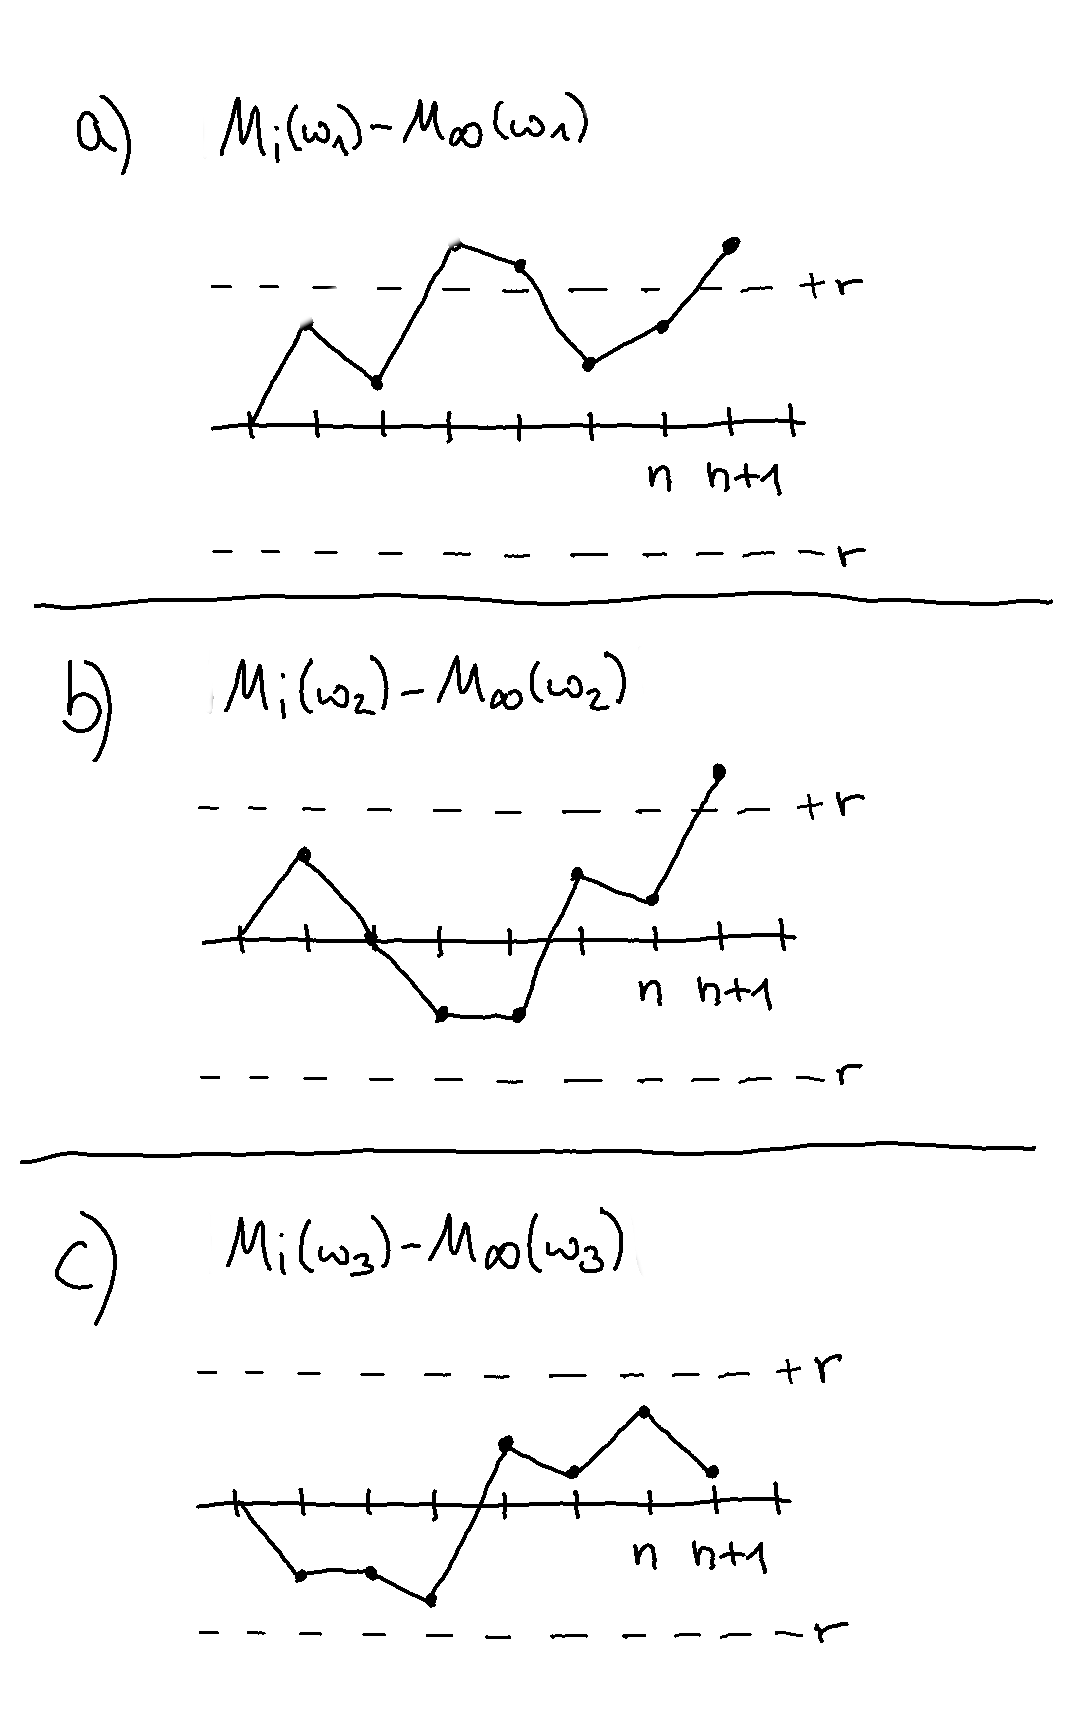
\includegraphics[width=0.75\textwidth]{pics/SketchUE1.png}
			\begin{enumerate}[label=Fall \alph{*})]
				\item \qquad $\omega_1 \in A_n \quad \rightarrow\quad \omega_1 \in A_{n+1}$
				\item \qquad $\omega_2 \not\in A_n \quad \rightarrow \quad \omega_2 \in A_{n+1}$
				\item \qquad $\omega_3 \not\in A_n \quad \rightarrow \quad \omega_3 \not\in A_{n+1}$
			\end{enumerate}
			$\omega \in A_n \quad \rightarrow \quad \omega \not\in A_{n+1} \quad$ nicht möglich $\implies A_n \subset A_{n+1} \quad\forall n\in\N$
			\label{AbbUEProzess}
	\end{figure}
	Außerdem brauchen wir noch die triviale Inklusion
	\begin{align*}
		\lbrace \omega : |M_n(\omega) - M_\infty(\omega)| \geq r\rbrace
		&\subset
		\lbrace \omega : \max\limits_{j\leq n} |M_j(\omega) - M_\infty(\omega)| \geq r\rbrace \\
		(&=\bigcup\limits_{j\leq n}\lbrace \omega : |M_j(\omega) - M_\infty(\omega)| \geq r\rbrace)
	\end{align*}
	Nun können wir endlich folgern:
	\begin{align*}
		\P\left[\lim\limits_{n\rightarrow\infty}|M_n-M_\infty| \geq r\right] 
		&\leq
		\P\left[\lim\limits_{n\rightarrow\infty}\max\limits_{j\leq n}|M_n-M_\infty| \geq r\right]  \\
		&=\lim\limits_{n\rightarrow\infty}\P\left[\max\limits_{j\leq n}|M_n-M_\infty| \geq r\right]  \\
		&\leq\lim\limits_{n\rightarrow\infty}\frac{\E\left[|M_n-M_\infty|\right]}{r}  \\
		&= 0 \qquad \forall r\geq 0
	\end{align*}
	Nun können wir die erste Aussage folgern
	\begin{align*}
		\P[\lim\limits_{n\rightarrow\infty}M_n \neq M_\infty]
		&=\P\left[\bigcup\limits_{k\in\N}\left\lbrace\lim\limits_{n\rightarrow\infty}|M_n-M_\infty| \geq \frac{1}{k}\right\rbrace\right] \\
		&\leq \sum\limits_{n\in\N}
		\P\left[\lim\limits_{n\rightarrow\infty}|M_n-M_\infty| \geq \frac{1}{k}\right] \\
		&\leq 0
	\end{align*}
	Also ist $M_\infty$ fast sicher der Grenzwert von $M_n$. Nun folgt der Rest sehr schnell mit dem Satz der dominierten Konvergenz, denn
	\begin{align*}
		\left.\begin{array}{c}
				M_n \stackrel{\text{f.s.}}{\rightarrow}M_\infty \\
				\|M_n\|_{L^p} \leq B 
			\end{array}\right\rbrace\implies M_n \stackrel{L^p}{\rightarrow}M_\infty
	\end{align*}
	Und somit folgt auch schlussendlich noch
	\begin{align*}
		\E\left[|M_\infty|^p\right] &= 
		\lim\limits_{n\rightarrow\infty}\E\left[|M_n|^p\right]  \\
		&\leq \sup\limits_{n\in\N}\E\left[|M_n|^p\right] \\
		&\leq B
	\end{align*}

\end{proof}


\end{document}
